\chapter{RÉSULTATS ET COMMENTAIRES}
\section{Introduction}
Dans ce chapitre, nous présentons les différents résultats obtenus après implémentation des algorithmes eigenfaces et Local Trinary Patterns. Pour cela, nous allons effectuer les tests sur les bases de données d'image ORL et YALE dans un premier temps, puis sur une base de donnée que nous allons créer.
\section{Bases de données de test}
\subsection{Base d'images ORL}\label{orl}
ORL est une base qui a été collectée entre avril 1992 et avril 1994 par le laboratoire AT\&T de
L'université  de Cambridge \footnote{http://web.mit.edu/emeyers/www/face\_databases.html\#orl consulté le 27/08/2016 à 22h36} . Elle est constituée de 40 personnes, chacune étant enregistrée sous 10 vues différentes. Les images sont de taille $112 \times 92$ pixels en format JPG et BMP
(portable  format  de  gris).  Pour  quelques  sujets,  les  images  ont  été  collectées  à  des  dates 
différentes,  avec  des  variations  dans  les  conditions  d'éclairage,  les  expressions  faciales 
(expression neutre, sourire et yeux fermés) et des occultations partielles par les lunettes. Toutes 
les  images  ont  été  collectées  sur  un  fond  foncé.  Les  poses  de  la  tête  présentent  quelques 
variations en profondeur par rapport à la pose frontale.

\begin{figure}[h]
 \caption[exemples d'images provenant de la base ORL]{exemples d'images provenant de la base ORL \\
source : http://web.mit.edu/emeyers/www/face\_databases.html\#orl}
	\centering
	
		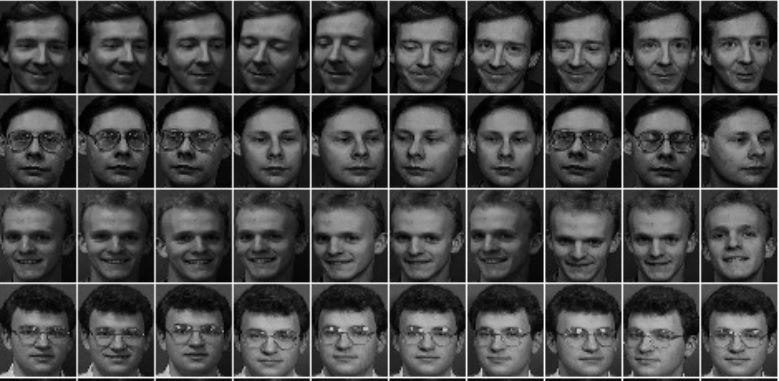
\includegraphics[width=450pt,height=250pt]{imagefromorl.JPG}
		
	\label{fig:imagefromorl}
\end{figure}
\newpage
\subsection{Base d'images YALE} \label{yale}

La base de données faciale Yale contient 165 images en niveaux de gris au format pgm de 15 personnes. Soit 11 images par sujet, les images ont chacune une expression du visage ou configuration différente : éclairage centrale, à gauche, à droite, port de verres ou non, heureux, triste, somnolent, surpris, et clin d'oeil.
\begin{figure}[htbp]
	\centering
		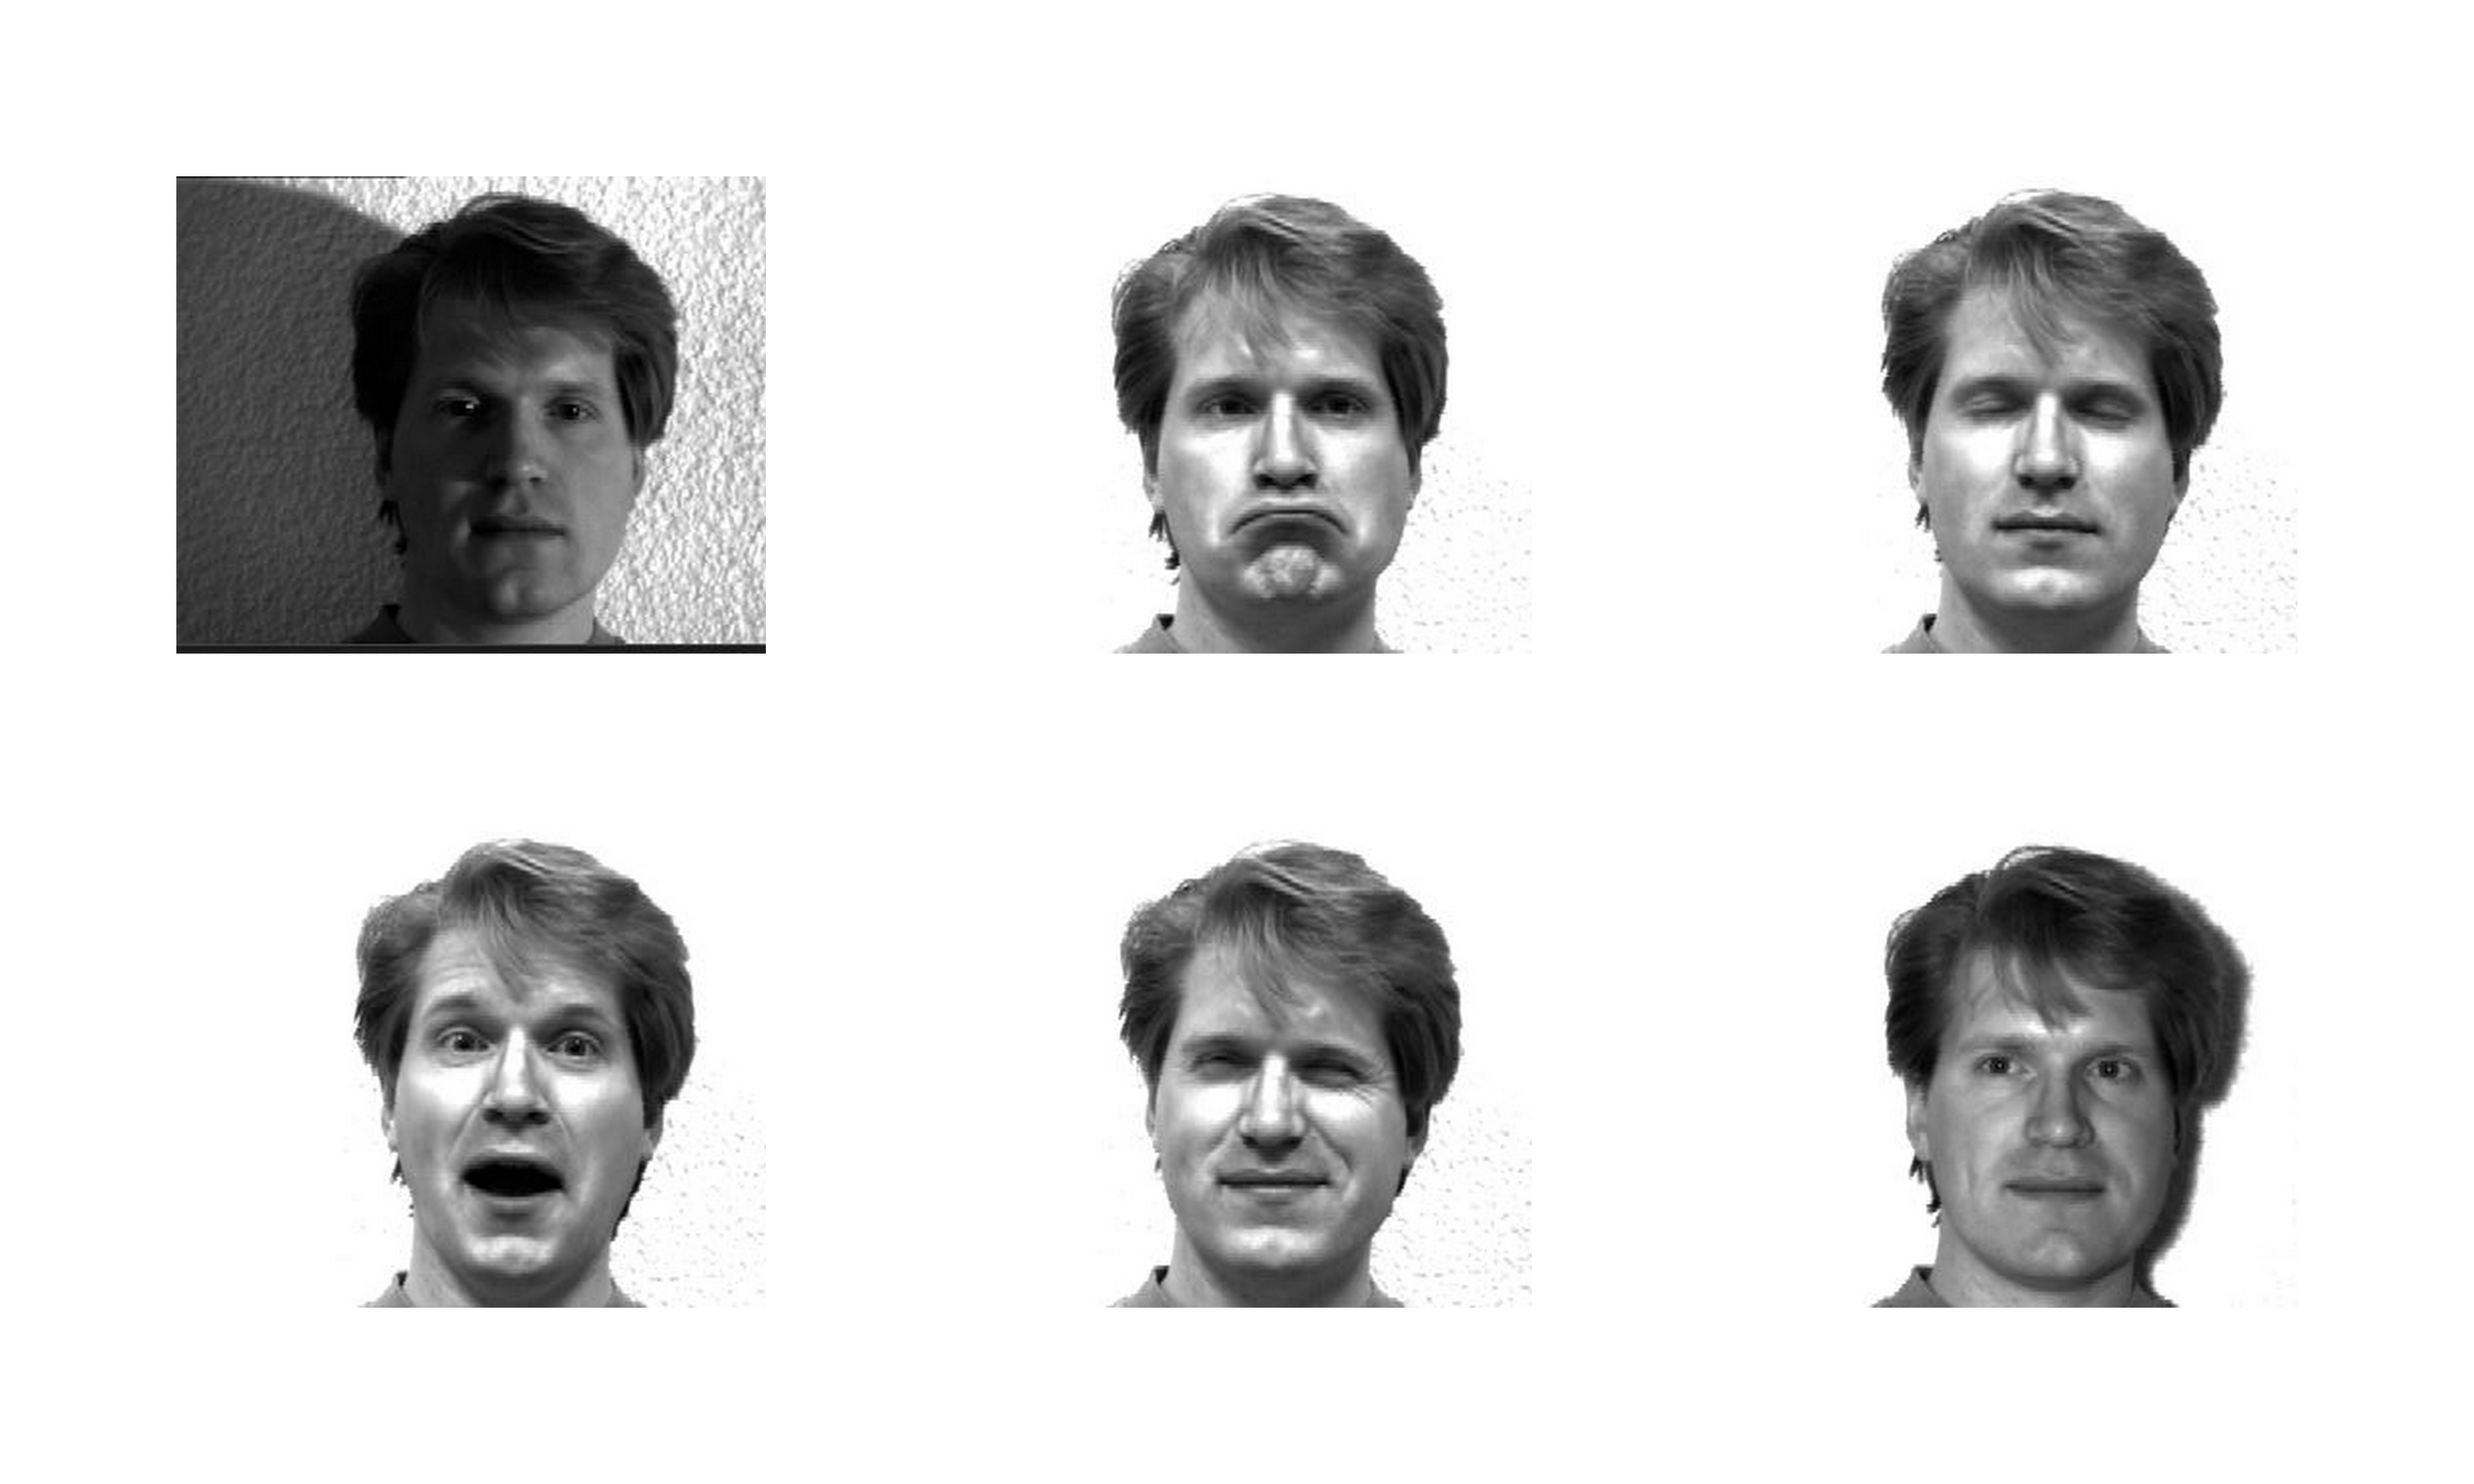
\includegraphics[width=450pt,height=200pt]{YAL.jpg}
		\caption[exemples d'images provenant de la base YALE ]{exemples d'images provenant de la base YALE \\
		source : http://web.mit.edu/emeyers/www/face\_databases.html\#yale}
	\label{fig:YAL}
\end{figure}

\subsection{Construire sa propre base de données d'images}
Pour construire une base de donnée d'images, on effectue des captures d'images de visage sur un ensemble d'individus. Ensuite on effectue un prétraitement (redimensionnement) sur l'ensemble des images capturées. Enfin les images sont groupées par dossiers en raison d'un individu par dossier.
\subsection{Séparation des bases de données}
Développer une application de reconnaissance faciale nécessite deux bases de données : une base de donnée d'apprentissage et une base de données pour les tests.
Dans les séries de test que nous avons effectué la base a été scindée de la façon suivante :
\begin{itemize}
	\item [\textbullet] Images apprentissages : Les 7 premières images servent pour la phase d'apprentissage.
	\item [\textbullet] Images Tests : Les 3 dernières images de chaque individu nous ont servies pour la réalisation des différents tests.
\end{itemize}
Le but est d'évaluer le taux de reconnaissance de  différents algorithmes présenté, en 
suivant un protocole de test basé sur la mesure de taux de reconnaissance. Le taux de reconnaissance est donné par l'expression 
$$taux\; de\; reconnaissance=\frac{nombre\; d'images\; de \;test\; reconnues}{nombre\; total\; d'images\; de \;test}$$
\section{Environnement de travail}

\subsection{Outils de développement}
Pour la réalisation de notre système de reconnaissance, nous avons utilisé le Java comme langage de programmation et la librairie OpenIMAJ. OpenIMAJ est un ensemble de librairies et d'outils pour l'analyse et la génération des contenus multimédia \footnote{http://www.openimaj.org}.  OpenIMAJ est principalement développé et maintenu par une équipe de chercheurs universitaires en électronique et d'informatique à l'Université de Southampton.
\nocite{OPEN}
\nocite{TUTO}
C'est possible d'écrire avec OpenIMAJ des programmes qui utilisent les bibliothèques dans toute langage JVM qui supporte
l'interopérabilité de Java, tel que Groovy, Jython, JRuby ou Scala. OpenIMAJ peut être exécuté même sur les téléphones Androïd et les tablettes.

OpenIMAJ est structurée en un grand nombre de librairies pouvant être utilisées de manière indépendantes. Les modules que nous avons utilisés sont : 
\begin{itemize}
	\item [\textbullet]  le module \textit{core} :  pour les modules qui contiennent les fonctionnalités usagée à travers les bibliothèques OpenIMAJ
	\item [\textbullet] le module \textit{core-image} : qui contient des définitions des images, les images élémentaires et les composants connectés.  Inclut le chargement, la sauvegarde et affichage des images.
	\item [\textbullet] le module \textit{core-vidéo} : qui contient des définitions d'un type de vidéo et fonctionnalités pour afficher et traiter des vidéos.
	\item [\textbullet]le module \textit{core-math} : mises en œuvre des outils mathématiques qui incluent géométrie, matrice et opérateurs statistiques.
		\item [\textbullet] le module \textit{image} : qui contient tout ce qui est relative aux images.
		\item [\textbullet] le module \textit{image-processing} : c'est une implémentation de nombreux algorithmes opérant sur les images comme la convolution, le redimensionnement, \ldots
		\item [\textbullet] le module \textit{image-local-features} :	qui contient des méthodes pour l'extraction de traits locaux
		\item [\textbullet] le module \textit{vidéo} : qui contient tout ce qui est relative aux flux vidéos.
		\item [\textbullet] le module \textit{vidéo-processing} : qui contient plusieurs fonctions de traitement de la vidéo.
		\item [\textbullet] le module \textit{machine-learning} : c'est un module dédiée à l'apprentissage automatique.
		\item [\textbullet] le module \textit{nearest-neighbour} : contient une implémentation de l'algorithme des K-plus proches voisins et autres méthodes d'approximation.
\end{itemize}
\section{Présentation de l'application}

Dans cette partie, nous présentons notre système de reconnaissance.
\subsection{Interface d'accueil}
C'est l'interface de communication entre les utilisateurs et le système de reconnaissance. Elle est assez intuitive et présente les différentes fonctionnalités du système (identification de visage, visage propre, suivi d'un visage, \ldots)
\begin{figure}[htbp]
	\centering
		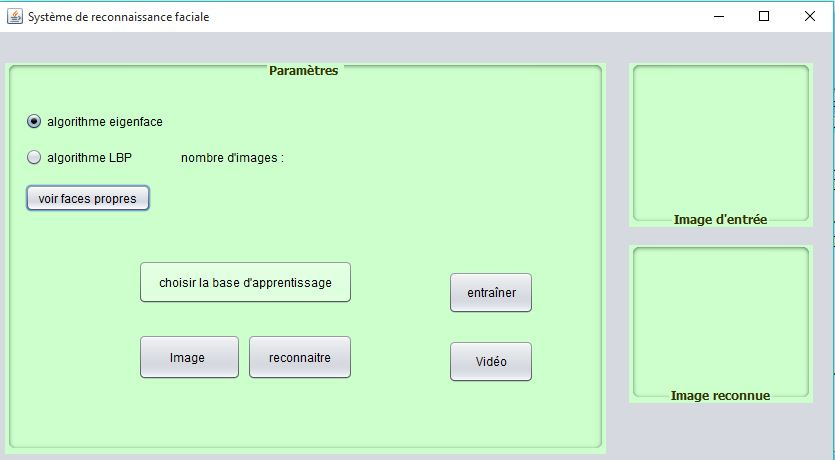
\includegraphics[width=450pt,height=350pt]{accueil.JPG}
	\caption{interface d'accueil du système de reconnaissance}
	\label{fig:accueil}
\end{figure}
\begin{itemize}
	\item [\textbullet]les boutons radio '\textit{algorithme eigenface}' et '\textit{algorithme LBP}' permettent de sélectionner l'algorithme de reconnaissance à utiliser.
	\item [\textbullet] Si l'algorithme eigenface est sélectionné, alors le bouton '\textit{voir faces propres}' apparaît. Ce dernier permet de voir les faces propres construites par la technique ACP.
	\item [\textbullet] le bouton '\textit{choisir la base d’apprentissage}' permet de charger la base de données d'images à utiliser.
	\item [\textbullet] une fois la base choisie, le bouton '\textit{entraîner}' permet d'entraîner l'algorithme de reconnaissance sur cette base.
	\item [\textbullet] le bouton '\textit{image}' permet de charger l'image d'entrée du système de reconnaissance. une fois l'image choisie, elle apparaît dans le panneau latéral droit à l'emplacement '\textit{image d'entrée}'
	\item [\textbullet] le bouton '\textit{reconnaître}' permet de lancer la reconnaissance.
	
	\item [\textbullet] le bouton '\textit{vidéo}' permet de lancer une reconnaissance en prenant comme entrée la vidéo capturée directement depuis un périphérique.
	\end{itemize}
	
	\subsection{Test de l'algorithme eigenface}
	
	\subsubsection{Sur la base de donnée ORL}
	\begin{enumerate}
		\item \textbf{Choix de la base d'apprentissage}
		
		\begin{figure}[htbp]
			\centering
				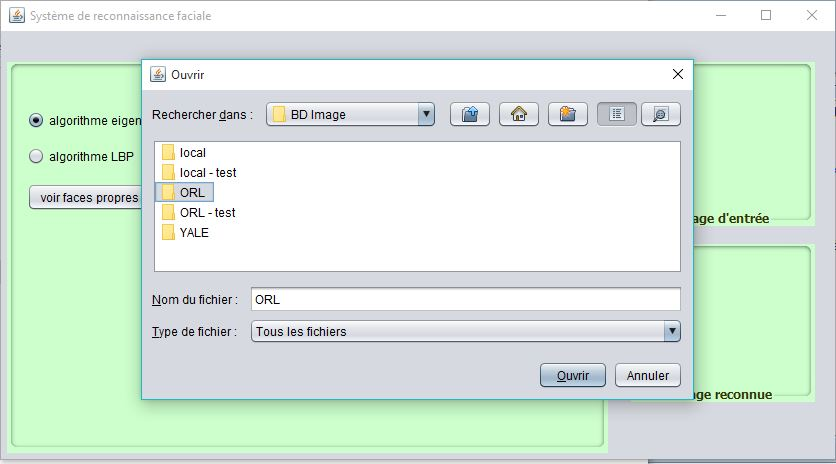
\includegraphics[width=450pt,height=350pt]{choixORL.JPG}
			\caption{choix de la base d'image ORL}
			\label{fig:choixORL}
		\end{figure}
		\newpage
			\item \textbf{entraînement de l'algorithme sur la base d'image}
			
			On sélectionne dans l'arborescence des fichiers le répertoire contenant la base de données ORL. Puis on clique sur le bouton '\textit{entraîner}'.
			\begin{figure}
				\centering
					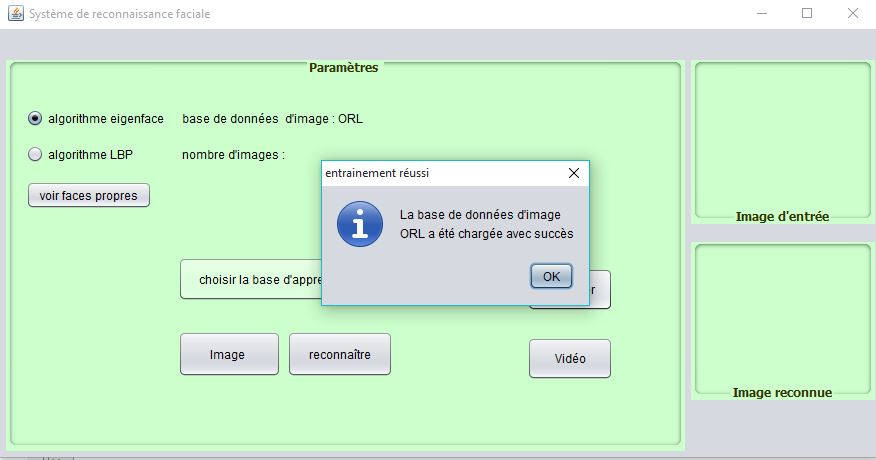
\includegraphics[width=450pt,height=350pt]{dbcharged.JPG}
				\caption{apprentissage de l'algorithme}
				\label{fig:dbcharged}
			\end{figure}
			\newpage
				\item \textbf{voir les faces propres.}
				
			Pour visualiser quelques faces propres de la base d'images, on sélectionne le bouton '\textit{voir faces propres}'
			
			\begin{figure}[htbp]
				\centering
					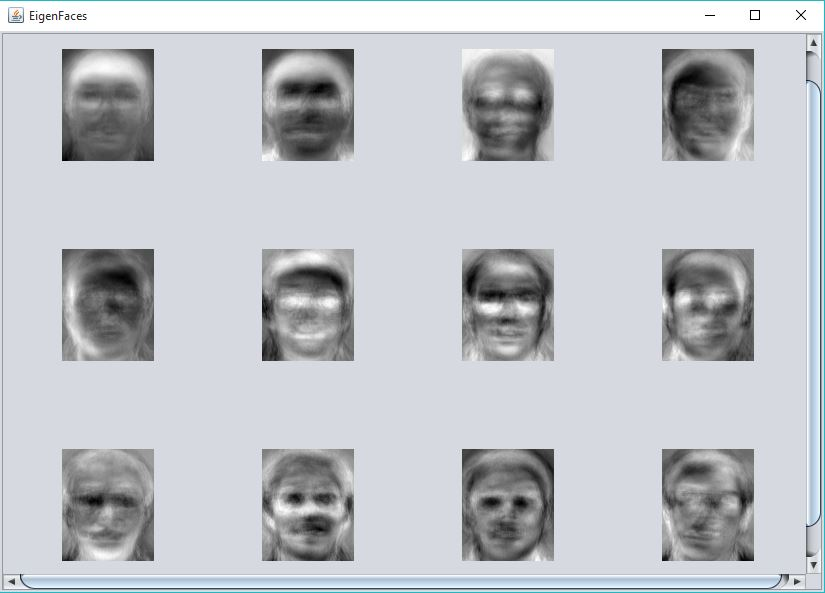
\includegraphics[width=450pt,height=350pt]{eigenORL.JPG}
				\caption{quelques faces propres de la base ORL}
				\label{fig:eigenORL}
			\end{figure}
			\newpage
			\item \textbf{identifier un visage.}
			
			Pour cela, cliquer sur le bouton '\textit{image}' et choisir l'image d'entrée. L'image d'entrée doit être de même taille que celles de la base d'apprentissage pour ce cas. 
			
			
			\begin{figure}[htbp]
				\centering
					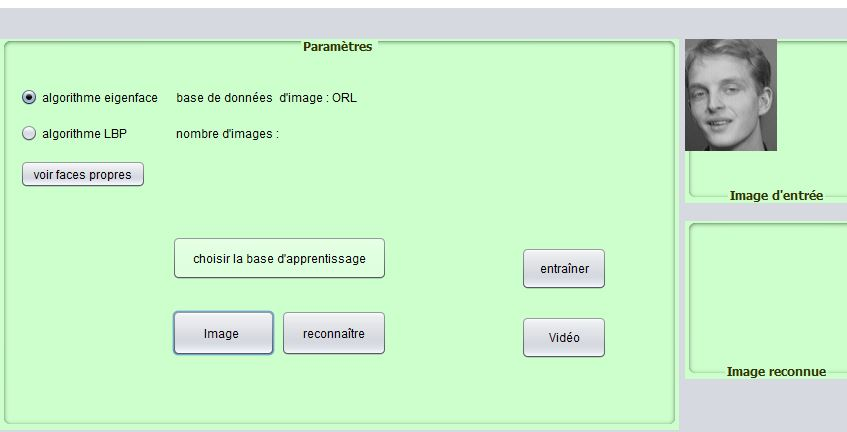
\includegraphics[width=450pt,height=220pt]{imageorlcharge.JPG}
				\caption{chargement d'une image de test}
				\label{fig:imageorlcharge}
			\end{figure}
		
	Puis on lance la reconnaissance en cliquant sur le bouton reconnaître.
			\begin{figure}[htbp]
				\centering
					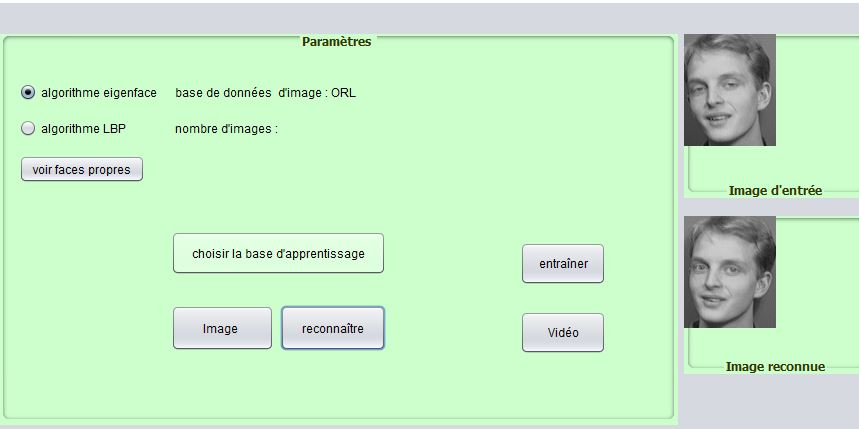
\includegraphics[width=450pt,height=220pt]{imageorlRecognize.JPG}
				\caption{visage reconnue}
				\label{fig:imageorlcharge}
			\end{figure}
		\end{enumerate}	
		
		 \subsubsection{Sur la base de donnée YALE}
		
		Le processus est le même que pour la base de donnée ORL, sauf que les images utilisés pour l'entraînement et le test proviennent de la base YALE. Un exemple de reconnaissance est représenté à la figure \ref{fig:eigenYale} .
		
		\begin{figure}[htbp]
			\centering
				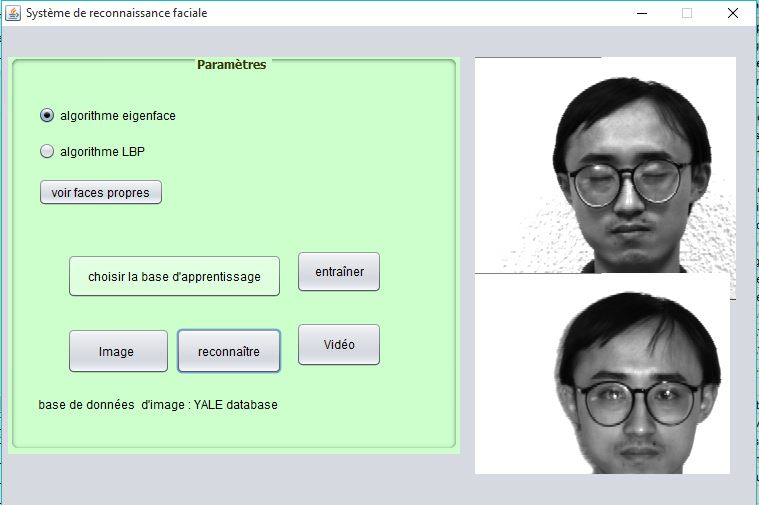
\includegraphics[width=400pt,height=200pt]{eigenYale.JPG}
			\caption{exemple de reconnaissance sur la base de données YALE}
			\label{fig:eigenYale}
		\end{figure}
			\subsection{Identifier un visage à partir d'un flux vidéo.}
			
			Pour cela, on choisit une base de donnée image potentielle. Dans ce cas, ça sera la base de donnée 'locale', puis on lance la reconnaissance en cliquant sur le bouton '\textit{video}'. La figure ci-dessous représente quelques images prélevées dans cette base.
			
			\begin{figure}[htbp]
				\centering
					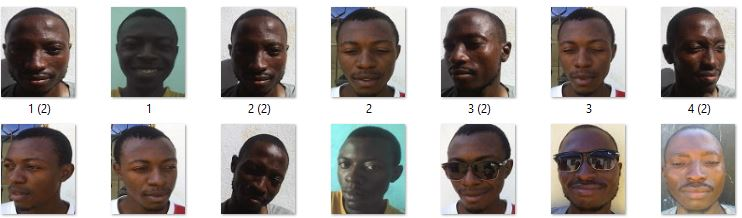
\includegraphics[width=450pt,height=170pt]{bdlocal.JPG}
				\caption{quelques images de la base de données 'local'}
				\label{fig:bdlocal}
			\end{figure}
					
			\begin{figure}[htbp]
				\centering
					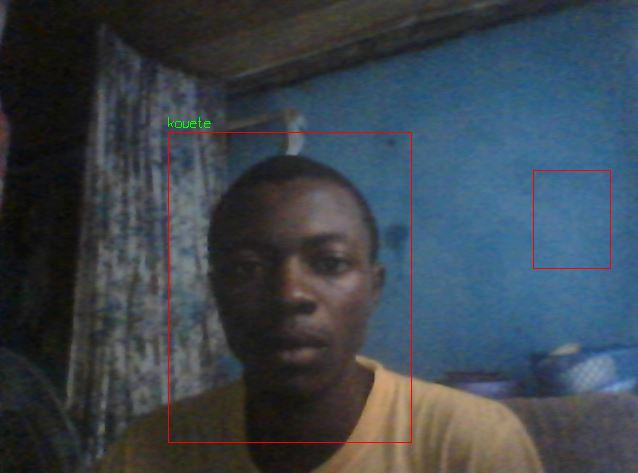
\includegraphics[width=350pt,height=200pt]{reconVideo.JPG}
				\caption{reconnaissance à partir d'un flux vidéo}
				\label{fig:reconVideo}
			\end{figure}
			
\newpage
	\subsubsection{Commentaires}
	Le taux de reconnaissance de l'algorithme eigenface sur la base de données ORL est de 93,20\% en moyenne pour une base d'entraînement de 6*40=240 images et une base de 4*40=160 pour les tests. Le temps d'apprentissage mesuré est d'environ 16 secondes contre un temps de reconnaissance d'environ une seconde. 
	
	Le même algorithme appliqué sur la base YALE séparée en une base de 6*15=90 images pour l'entraînement et une base de 5*15=75 images pour les tests donne un taux de reconnaissance de 78.67\% en moyenne.  Le temps d'apprentissage mesuré est d'environ 24 secondes contre un temps de reconnaissance de 14 secondes. 
	
		\subsection{Test de l'algorithme LBP}
Les tests se déroulent de la même manière que pour l'algorithme eigenface. Il suffit d'activer le bouton radio 'algorithme LBP' pour choisir d'utiliser l'algorithme LBP. Des exemples de test sont illustrés par les figures \ref{fig:reconLBP1} et \ref{fig:reconLBP2} ci-dessous.		
		\begin{figure}[htbp]
			\centering
				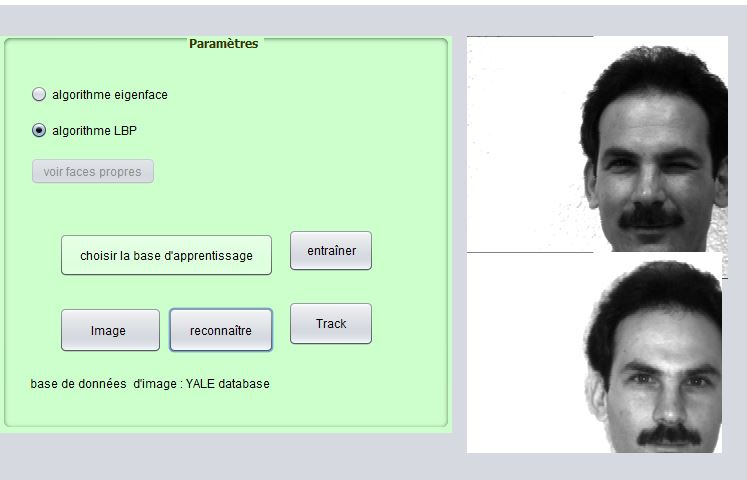
\includegraphics[width=350pt,height=200pt]{reconLBP1.JPG}
			\caption{algorithme LBP appliqué sur la base YALE}
			\label{fig:reconLBP1}
		\end{figure}	
		
		\begin{figure}[htbp]
			\centering
				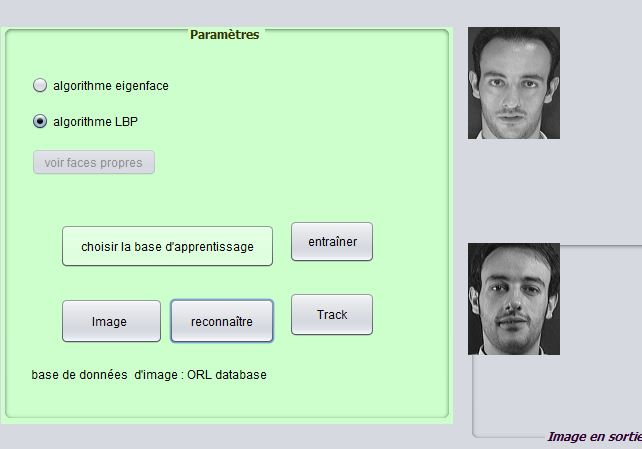
\includegraphics[width=350pt,height=250pt]{reconLBP2.JPG}
			\caption{algorithme LBP appliqué à la base ORL}
			\label{fig:reconLBP2}
		\end{figure}
		\newpage
	L'un des points forts de l'algorithme LBP est sa capacité à pouvoir opérer sur des bases d'images constituées d'un seul échantillon. Cet avantage peut être utilisé pour pister un individu par un réseau de caméra. Une application est illustrée par les captures suivantes :
	
	\begin{enumerate}
		\item Dans un premier temps, le système détecte le visage. Ce dernier peut alors être enregistré en faisant une combinaison des touches Ctrl et S.
		\begin{figure}[htbp]
		\centering
			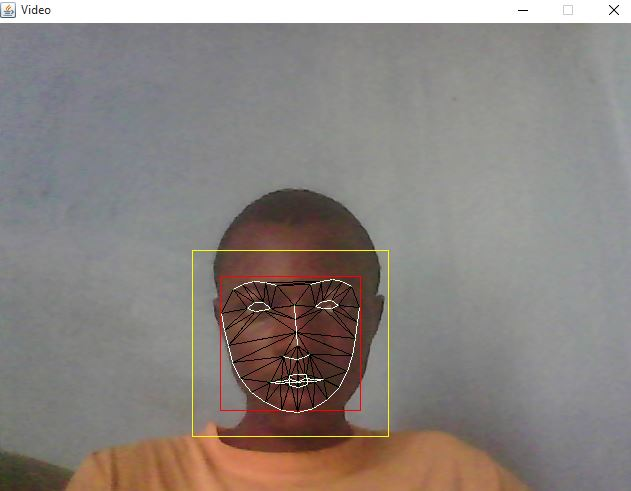
\includegraphics[width=350pt,height=200pt]{track1.JPG}
		\caption{détection et capture du visage}
		\label{fig:track 1}
	\end{figure}
	\item L'utilisateur entre une information caractérisant le visage capturée, puis valide. Le système s'entraîne alors à reconnaître le visage enregistré. Par exemple un nom.
	\begin{figure}[htbp]
		\centering
			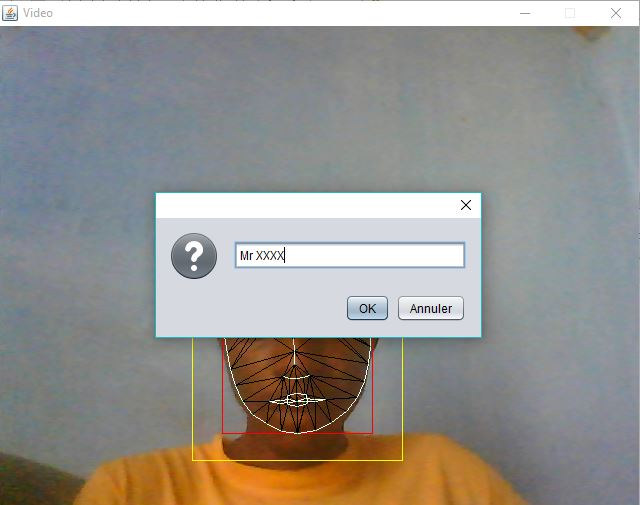
\includegraphics[width=350pt,height=200pt]{track2.JPG}
		\caption{enregistrement du visage}
		\label{fig:track 1}
	\end{figure}
	
	\item Le visage est alors reconnu à chaque fois qu'il passe dans le champ de vision du périphérique de capture.
	
	\begin{figure}[htbp]
		\centering
			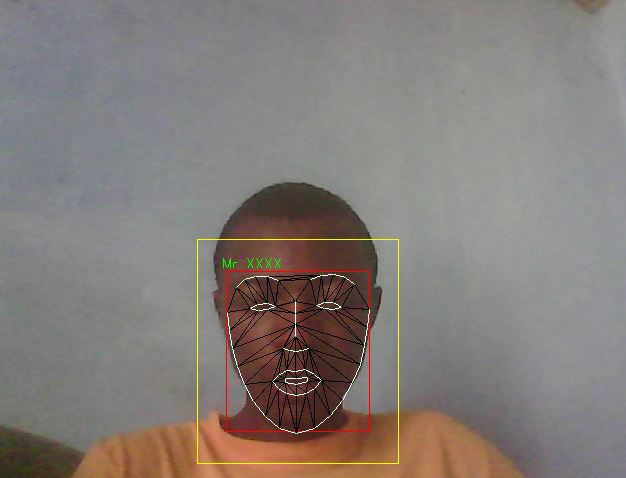
\includegraphics[width=350pt,height=200pt]{track3.JPG}
		\caption{suivi du visage}
		\label{fig:track 1}
	\end{figure}
	\end{enumerate}
	
	
	
		\subsubsection{Commentaires}
	Le taux de reconnaissance de l'algorithme LBP sur la base de données ORL est de 96.6\% pour les mêmes bases d'apprentissage et de test que précédemment. Le temps d'apprentissage mesuré est d'environ 22 secondes contre un temps de reconnaissance d'environ 13 secondes. 
	
	Le même algorithme appliqué sur la base YALE séparée en une base de 7*15=105 images pour l'entraînement et une base de 4*15=760 images pour les tests donne un taux de reconnaissance de 46.67\% seulement. Ceci est du au fait que les images de la base YALE présentent de variations extérieures. Le temps d'apprentissage mesuré est d'environ 16 secondes contre un temps de reconnaissance de 8 secondes. 
	\subsection{Comparaison des performances}
	Le tableau ci-dessous est une comparaison des performances des algorithmes eigenface et LBP sur les bases de données ORL et YALE.
	
	\begin{table}[htbp]
		\centering
			\begin{tabular}{|l|c|c |}
				\hline &algorithme eigenface& algorithme LBP\\
				\hline ORL  & 93.2\%& 96.6\%\\
				\hline YALE & 78.67\%& 46.67\%\\
				\hline
			\end{tabular}
		\caption{performance des algorithmes LBP et eigenface sur les bases d'images ORL et YALE}
		\label{tab:performanceDesAlgorithmesLBPEtEigenfaceSurLesBasesDImagesORLEtYALE}
	\end{table}
\section{Conclusion}
Nous avons présenté dans ce chapitre les différents résultats obtenus après implémentation et tests des algorithmes LBP et eigenfaces. Les bases de données d'images sont ORL( section \ref{orl}), YALE (\ref{yale}) et une base nommée 'local' que nous avons nous même créée. Il est à noter que le temps d'exécution des algorithmes croît avec le nombre d'image contenue dans la base de données. Par ailleurs l'algorithme LBP s'avère un peu plus rapide et est mieux adapté pour le problème à un échantillon.
\nocite{TRACK}